\section{Results}
\label{sec:results}

\subsection{The Federation Being Valued}
\label{sec:federation}
Our re-implementation reproduces the base study's released code to within $1.2\times10^{-14}$, and its sustainability finding holds under our protocol: joining brings no significant average gain over local training (FL$-$LOC $=\pDFLminusLOC$) and a free-rider obtains almost the same model (FR$-$FL $=\pDFRminusFL$). DP changes the mean per-hospital AUC by only $\pDpLossHalf$ at $\varepsilon=0.5$ for this seven-parameter model. The model transports to held-out countries in discrimination but not in calibration (O/E \pOeMin--\pOeMax), which an intercept update on 20\% of a new country's patients largely fixes (Supplementary Section~\ref{S-sec:pca19_more}).

\subsection{Retraining Spends the Budget Hundreds of Times}
\label{sec:p19_retrain}
\label{sec:p19_osa}
Retraining every coalition of the ten largest hospitals at a per-run $\varepsilon$ looks accurate (Spearman $\rho=\pShRhoTen$ with the non-private ranking at $\varepsilon=10$, \pShRhoTwo{} at $\varepsilon=2$), but each hospital joins 512 runs, so a per-run $\varepsilon$ of 10, 5 or 1 is a total of about \trueEpsTen{}, \trueEpsFive{} and \trueEpsOne{} (Supplementary Table~\ref{S-tab:osa}). Held at the stated total (\emph{budget-matched}), $\rho$ falls to \bmRhoTen{} at $\varepsilon=10$ and \bmRhoOne{} at $\varepsilon=1$. OSA-Shapley spends the budget once and keeps $\rho=\osaNoDP$ without DP, \osaRhoTwo{} at $\varepsilon=2$ and \osaRhoOne{} at $\varepsilon=1$; at $\varepsilon=2$ it beats budget-matched retraining by $\osaVsBmTwo$ and matches per-run retraining ($\osaVsPrTwo$), which spends 28--42 times more privacy. All 19 hospitals can be valued exactly: the DP ranking agrees with the non-private one at $\rho=\osaNineRhoFive$ ($\varepsilon=5$) and \osaNineRhoOne{} ($\varepsilon=1$).

\subsection{Against Reconstruction and Cheap Proxies}
\label{sec:p19_post}
\label{sec:p19_proxies}
For the ten largest hospitals OSA-Shapley is more accurate than exact MR at every budget ($\rho$ \osaRhoTwo{} vs \mrRhoTwo{} at $\varepsilon=2$, difference \osaVsMrTwo; \osaRhoOne{} vs \mrRhoOne{} at $\varepsilon=1$) and beats OR by \osaVsOrTwo{} (Table~\ref{tab:proxies}; Supplementary Table~\ref{S-tab:osa_post}). The gap exists without DP ($\rho$ \osaNoDP{} vs \mrRhoNoDP), so it comes from the coalition proxy, not the noise.

Cheap proxies carry almost no information here: size, case counts and summary statistics reach $\rho$ \pxLSizeNoDP, \pxLPosNoDP{} and \pxLStatNoDP{} (OSA$-$size $=\pxdLSizeTwo$ at $\varepsilon=2$), because these hospitals differ in case mix and their value depends on what the others provide; a self-reported AUC is unverifiable and weak ($\rho=\pxLOwnTwo$). A score built on the released models is much better: the single-release AUC reaches $\rho=\pxLRefTwo$ at $\varepsilon=2$, and OSA-Shapley is comparable there ($\pxdLRefTwo$) and better at $\varepsilon=1$ ($\pxdLRefOne$), at no extra privacy cost and with values that are proper Shapley values. 

\begin{table*}[t]
\caption{Is OSA-Shapley worth its cost? Agreement (Spearman $\rho$) of cheap contribution proxies and of privacy-honest valuations with the exact non-private retraining Shapley ranking, on real PCa-19 hospitals (20 held-out splits). \emph{What is shared}: what each hospital must reveal. Proxies that use a model use the same DP releases as OSA-Shapley and therefore cost the same $\varepsilon$; size, counts and statistics are shared without DP. \emph{Useless}: share of splits in which a hospital whose training labels were replaced by random labels (es6) is ranked last at $\varepsilon=2$; a tie for last place does not count.}
\centering\scriptsize
\setlength{\tabcolsep}{4pt}
\begin{tabular}{llccccccc}
\toprule
 & & \multicolumn{4}{c}{Ten largest hospitals} & \multicolumn{3}{c}{Ten smallest hospitals} \\
\cmidrule(lr){3-6}\cmidrule(lr){7-9}
Contribution score & What is shared & no DP & $\varepsilon=2$ & $\varepsilon=1$ & Useless & no DP & $\varepsilon=2$ & $\varepsilon=1$ \\
\midrule
Hospital size $n_k$ & size (public) & 0.08 & 0.08 & 0.08 & 0\% & 0.74 & 0.74 & 0.74 \\
Number of csPCa cases & one count & 0.02 & 0.02 & 0.02 & 0\% & 0.50 & 0.50 & 0.50 \\
Similarity of summary statistics & feature means, prevalence & \ensuremath{-}0.18 & \ensuremath{-}0.18 & \ensuremath{-}0.18 & 0\% & 0.72 & 0.72 & 0.72 \\
Self-reported local AUC & one AUC (unverifiable) & 0.36 & 0.25 & 0.26 & 100\% & 0.40 & 0.54 & 0.56 \\
Single-model AUC on reference set & one DP model ($\varepsilon$) & 0.93 & 0.85 & 0.71 & 100\% & 0.94 & 0.79 & 0.72 \\
Leave-one-out of averaged models & one DP model ($\varepsilon$) & 0.85 & 0.77 & 0.74 & 0\% & 0.59 & 0.34 & 0.34 \\
OR reconstruction & DP-FedAvg run ($\varepsilon$) & 0.42 & 0.51 & 0.50 & 100\% & 0.79 & 0.74 & 0.59 \\
MR reconstruction (GTG bound) & DP-FedAvg run ($\varepsilon$) & 0.74 & 0.75 & 0.65 & 70\% & 0.86 & 0.78 & 0.74 \\
Retraining, budget-matched & $2^{K-1}$ runs ($\varepsilon$) & -- & 0.18 & 0.10 & 60\% & -- & 0.45 & 0.29 \\
\textbf{OSA-Shapley (ours)} & one DP model ($\varepsilon$) & \textbf{0.96} & \textbf{0.89} & \textbf{0.80} & 100\% & \textbf{0.95} & \textbf{0.79} & \textbf{0.68} \\
\bottomrule
\end{tabular}
\label{tab:proxies}
\end{table*}


\subsection{Small Hospitals}
To study small silos without simulating any, we value the ten smallest PCa-19 hospitals (\pxSmallMin--\pxSmallMax{} patients). Without DP OSA-Shapley is again the most accurate valuation ($\rho=\pxSOsaNoDP$; OSA$-$MR $=\pxdSMrNoDP$). Under DP its advantage disappears: at $\varepsilon=2$ OSA and MR agree with the ranking equally well (\pxSOsaTwo{} and \pxSMrTwo), and at $\varepsilon=1$ MR is slightly, not significantly, ahead (\pxdSMrOne); budget-matched retraining remains far worse ($\rho=\pxSBmTwo$). Here contribution follows volume, and size alone reaches $\rho=\pxSSizeNoDP$ (OSA$-$size $=\pxdSSizeTwo$ at $\varepsilon=2$). This is the regime Proposition~3 predicts: the release of a hospital with a few dozen patients carries noise of order $\sigma/n_k$, whereas reconstruction averages over the federation in every round.

\subsection{Useless Data and a Non-Convex Model}
\label{sec:p19_robust}
\label{sec:p19_small}
\label{sec:p19_mlp}
A hospital whose training labels were replaced by random labels (\corrHosp) is ranked last by the non-private reference in \corrTruth{} of splits; at $\varepsilon=2$ and 1 by OSA-Shapley in \corrOsaTwo{} and \corrOsaOne, by MR in \corrMrTwo{} and \corrMrOne, by budget-matched retraining in \corrBmTwo{} and \corrBmOne, and never by size or statistics. With a federated one-hidden-layer MLP (16 units; coalition prediction = size-weighted average of members' log-odds), OSA-Shapley is the most accurate valuation without DP ($\rho=\mlpOsaNoDP$ vs \mlpMrNoDP{} for MR) but loses under DP (\mlpOsaTwo{} vs \mlpMrTwo{} at $\varepsilon=2$; OSA$-$MR $=\mlpOsaVsMrTwo$): a network trained alone for 200 noisy steps accumulates the perturbation, whereas MR's short updates restart from the shared model every round (Supplementary Table~\ref{S-tab:osa_mlp}).

\subsection{A Second Real Federation: Heart Disease}
\label{sec:heart}
Without DP the heart-disease federation confirms the picture: OSA-Shapley recovers the exact ranking best ($\rho=\hrOsaNoDP$ vs \hrMrNoDP{} for MR; OSA$-$MR $=\hrdMrNoDP$; Table~\ref{tab:heart}). Under DP it does not. The hospitals have 98--242 training patients for 21 parameters and nearly equal contributions (Shapley values \hrPhiMin--\hrPhiMax{} AUC), so release noise dominates: at $\varepsilon=2$ MR is better (\hrMrTwo{} vs \hrOsaTwo; OSA$-$MR $=\hrdMrTwo$), and at $\varepsilon=1$ no valuation beats chance. Retraining does not help even at its modest composed cost here (a stated $\varepsilon=2$ costs \hrTrueTwo). Size is anti-correlated with contribution ($\rho=\hrSizeNoDP$), whereas OSA-Shapley and the single-release score still rank \hrCorrupt{} with random labels last in \hrCOsaTwo{} and \hrCRefTwo{} of splits at $\varepsilon=2$.

\begin{table}[t]
\caption{Second real federation: the four hospitals of the UCI Heart Disease collection (Cleveland (303), Budapest (294), Zurich/Basel (123), Long Beach VA (200) patients), coronary artery disease, 20 held-out splits. Spearman $\rho$ with the exact non-private retraining Shapley ranking; with four hospitals $\rho$ moves in steps of 0.2. Per-run retraining really costs $\varepsilon\approx16$, 6.1 and 2.9 at a stated 5, 2 and 1. \emph{Useless}: share of splits in which Budapest, given random training labels, is ranked last at $\varepsilon=2$.}
\centering\scriptsize
\setlength{\tabcolsep}{3pt}
\begin{tabular}{lccccc}
\toprule
Contribution score & no DP & $\varepsilon=5$ & $\varepsilon=2$ & $\varepsilon=1$ & Useless \\
\midrule
Hospital size $n_k$ & \ensuremath{-}0.38 & \ensuremath{-}0.38 & \ensuremath{-}0.38 & \ensuremath{-}0.38 & 0\% \\
Similarity of summary statistics & \ensuremath{-}0.38 & \ensuremath{-}0.38 & \ensuremath{-}0.38 & \ensuremath{-}0.38 & 0\% \\
Self-reported local AUC & \ensuremath{-}0.18 & \ensuremath{-}0.17 & \ensuremath{-}0.31 & \ensuremath{-}0.30 & 70\% \\
Single-model AUC on reference set & 0.76 & 0.42 & \ensuremath{-}0.04 & \ensuremath{-}0.34 & 100\% \\
Leave-one-out of averaged models & 0.82 & 0.69 & 0.42 & 0.18 & 85\% \\
OR reconstruction & 0.23 & 0.29 & 0.18 & 0.04 & -- \\
MR reconstruction (GTG bound) & 0.70 & 0.64 & 0.45 & \ensuremath{-}0.35 & -- \\
Retraining, per run & -- & 0.34 & \ensuremath{-}0.09 & \ensuremath{-}0.27 & -- \\
Retraining, budget-matched & -- & \ensuremath{-}0.02 & \ensuremath{-}0.18 & \ensuremath{-}0.15 & -- \\
\textbf{OSA-Shapley (ours)} & \textbf{0.92} & \textbf{0.51} & \textbf{0.15} & \textbf{\ensuremath{-}0.18} & 100\% \\
\bottomrule
\end{tabular}
\label{tab:heart}
\end{table}


\section{A Decision Rule, Tested in Advance}
\label{sec:rule}
By Proposition~3 the noise norm of a release over $p$ parameters scales as $\sqrt p/n_k$, so we index a setting by $\nu$, the median training patients per hospital divided by $\sqrt p$. OSA-Shapley won at $\nu=\nuLarge$ (ten largest PCa-19 hospitals) and not at $\nu\le\nuSmall$ (ten smallest \nuSmall, heart \nuHeart, MLP \nuMlp; Supplementary Table~\ref{S-tab:decision}), suggesting a switch-over between $\nu\approx50$ and 100.

\emph{Internally pre-registered test.} A threshold read off the results it explains is not evidence. Before running a new experiment we wrote down its design and six hypotheses and fixed them by a SHA-256 hash (Supplementary Section~\ref{S-sec:prereg}); the registration is internal, not public, and was written and run on the same day, so its timing cannot be verified independently and we treat the test as a prospectively specified internal check rather than a formal pre-registration. Within the ten largest hospitals we lowered $\nu$ by keeping 60--15\% of the training patients (arm A) or adding 21--100 uninformative features (arm B), each condition with its own exact reference (Fig.~\ref{fig:nu}).

The direction held but the threshold did not. As predicted, OSA-Shapley beat MR at $\nu\ge100$ (H1), its advantage shrank with $\nu$ (H3; Spearman \nsSpear), both arms agreed in sign (H5), and stronger privacy moved the switch-over up (H6). Contrary to H2 and H4, it kept a significant advantage down to $\nu\approx\nsAFortyFiveNu$ (OSA$-$MR $=\nsAFortyFiveTwo$ at $\varepsilon=2$) and fell behind only at $\nu\approx\nsASeventeenNu$; the mean difference changed sign at $\nu\approx\nsCrossTwo$ ($\varepsilon=2$) and \nsCrossOneMin--\nsCrossOneMax{} ($\varepsilon=1$). Four of six hypotheses held, and we revise the rule:

\begin{figure}[!t]
\centering
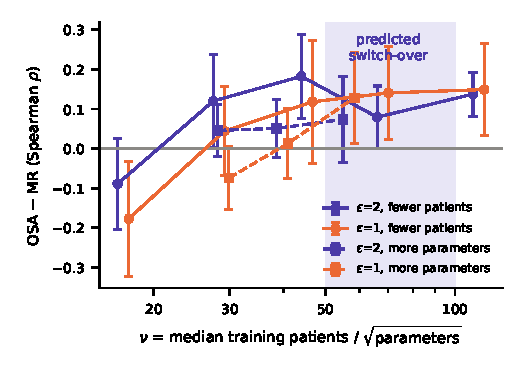
\includegraphics[width=\columnwidth]{figures/figure20_nu_sweep.pdf}
\caption{Internally pre-registered test: OSA$-$MR (paired difference in Spearman $\rho$ with the exact reference, 95\% CI, 20 splits) as $\nu$ is lowered within the ten largest PCa-19 hospitals, by removing patients (solid) or adding uninformative parameters (dashed). Shaded: the switch-over predicted before the test.}
\label{fig:nu}
\end{figure}

\begin{enumerate}
    \item \emph{Count the cost} of any valuation (Proposition~2); never retrain coalitions at a per-run budget.
    \item \emph{Without DP on the releases}, use OSA-Shapley, the most accurate valuation in all four settings.
    \item \emph{Under DP with a convex model}, OSA-Shapley is at least as accurate as MR down to $\nu\approx30$ ($\varepsilon=2$) and 40 ($\varepsilon=1$); below that use MR, which adds no cost when the federation trains with DP-FedAvg. \emph{With a non-convex model}, use MR.
    \item \emph{Check size before using it}: it matched contribution only where hospitals differed mainly in volume, and never detects bad data; a single released model's score does.
    \item \emph{When in doubt, compute both.} The heart-disease federation ($\nu=\nuHeart$) favoured MR although the sweep says OSA should be competitive; four hospitals make $\rho$ coarse and site-specific missing data leave single-hospital models poorly determined, both untested explanations. With small $\nu$ at $\varepsilon\le1$, equal shares plus screening for bad data is the honest fallback.
\end{enumerate}
